\documentclass[12pt,a4paper]{article}
\usepackage[margin=1in]{geometry}
\usepackage{booktabs}
\usepackage{threeparttable}
\usepackage{float}
\usepackage{amsmath,amssymb}
\usepackage{graphicx}
\usepackage{caption}
\usepackage[colorlinks=true,linkcolor=blue,citecolor=blue]{hyperref}
\usepackage{setspace}
\onehalfspacing

\title{Cross-Sectional Crypto Return Predictability\\and Volatility Spillovers}
\author{econtools Research Pipeline}
\date{\today}

\begin{document}
\maketitle

\begin{abstract}
Using a panel of 417 cryptocurrencies over 11 years,
we study the cross-sectional determinants of daily altcoin returns and
test for BTC-to-altcoin volatility spillovers. We compare inference
under HC1, HC3, and HAC covariance estimators, and implement
Fama-MacBeth monthly cross-sectional regressions. We find strong
contemporaneous co-movement with BTC but limited predictive power
from lagged characteristics, and document significant volatility
transmission from BTC to the altcoin market.
\end{abstract}

\section{Introduction}

Cryptocurrency markets present a unique laboratory for cross-sectional
asset pricing research. Unlike equity markets, where hundreds of ``anomalies''
have been documented, the cross-section of expected crypto returns remains
relatively unexplored. Key questions include: does size (market capitalisation)
predict returns? Is there a momentum effect? Does illiquidity command a premium?

We address these questions with pooled panel OLS using multiple robust
standard error estimators, supplemented by Fama-MacBeth (1973) monthly
cross-sectional regressions that allow time variation in risk premia.

\section{Data}

Our panel comprises 1,019,201 daily observations across 417 altcoins
(excluding BTC, which serves as the market factor). We require at least
730 days of price history and exclude returns exceeding 100\% in absolute
value as likely data errors.

\section{Cross-Sectional Return Predictors}

\begin{table}[htbp]
\centering
\caption{Cross-Sectional Determinants of Altcoin Returns}
\label{tab:cross_section}
\begin{threeparttable}
\resizebox{\textwidth}{!}{%
\small{%
\begin{tabular}{l c c c c c}
\toprule
 & (1) & (2) & (3) & (4) & (5) \\
 & OLS & OLS & OLS & OLS & OLS \\
\midrule
\multicolumn{6}{l}{\textit{Market exposure}} \\[2pt]
\$r^{BTC}\_t\$ & -0.042$^{\ast\ast\ast}$ &  & -0.042$^{\ast\ast\ast}$ & -0.042$^{\ast\ast\ast}$ & -0.042$^{\ast\ast\ast}$ \\
 & $(0.003)$ &  & $(0.003)$ & $(0.003)$ & $(0.003)$ \\
\$r^{BTC}\_{t-1}\$ & 0.034$^{\ast\ast\ast}$ &  & 0.039$^{\ast\ast\ast}$ & 0.039$^{\ast\ast\ast}$ & 0.039$^{\ast\ast\ast}$ \\
 & $(0.003)$ &  & $(0.003)$ & $(0.003)$ & $(0.003)$ \\
\addlinespace[2pt]
\multicolumn{6}{l}{\textit{Characteristics}} \\[2pt]
\$\ln(\text{MCap})\_{t-1}\$ &  & -0.000$^{\ast}$ & -0.000 & -0.000 & -0.000 \\
 &  & $(0.000)$ & $(0.000)$ & $(0.000)$ & $(0.000)$ \\
\$\text{Mom}\_{7d,t-1}\$ &  & -0.007$^{\ast\ast\ast}$ & -0.006$^{\ast\ast\ast}$ & -0.006$^{\ast\ast\ast}$ & -0.006$^{\ast\ast\ast}$ \\
 &  & $(0.001)$ & $(0.001)$ & $(0.001)$ & $(0.001)$ \\
\$\text{Mom}\_{30d,t-1}\$ &  & 0.002$^{\ast\ast\ast}$ &  &  &  \\
 &  & $(0.000)$ &  &  &  \\
\$\ln(\text{Volume})\_{t-1}\$ &  &  & -0.000 & -0.000 & -0.000 \\
 &  &  & $(0.000)$ & $(0.000)$ & $(0.000)$ \\
\$\sigma\_{30d,t-1}\$ &  &  & -0.000$^{\ast}$ & -0.000$^{\ast}$ & -0.000$^{\ast\ast}$ \\
 &  &  & $(0.000)$ & $(0.000)$ & $(0.000)$ \\
\$\ln(\text{Amihud})\_{t-1}\$ &  &  & -0.000 & -0.000 & -0.000 \\
 &  &  & $(0.000)$ & $(0.000)$ & $(0.000)$ \\
\addlinespace[2pt]
\midrule
$N$ & 1019201 & 1019201 & 1019201 & 1019201 & 1019201 \\
$R^2$ & 0.000 & 0.000 & 0.001 & 0.001 & 0.001 \\
Adj.\ $R^2$ & 0.000 & 0.000 & 0.001 & 0.001 & 0.001 \\
SE type & HC1 & HC1 & HC1 & HC3 & HAC \\
\bottomrule
\end{tabular}
%}
}
\begin{tablenotes}
\footnotesize
\item Dependent variable: next-day log return $r_{i,t+1}$ for altcoin $i$.
\item Panel of altcoins (excluding BTC) with $\geq$730 days of data.
\item Columns (1)--(3): HC1 SEs; Column (4): HC3 SEs; Column (5): HAC(5) SEs.
\item ${}^{*}p<0.10$, ${}^{**}p<0.05$, ${}^{***}p<0.01$.
\end{tablenotes}
\end{threeparttable}
\end{table}

The contemporaneous BTC return ($r^{BTC}_t$) is the strongest predictor,
reflecting the high correlation structure of crypto markets. Among lagged
characteristics, momentum and market capitalisation show the most consistent
effects, though magnitudes are small.

\begin{figure}[H]
\centering
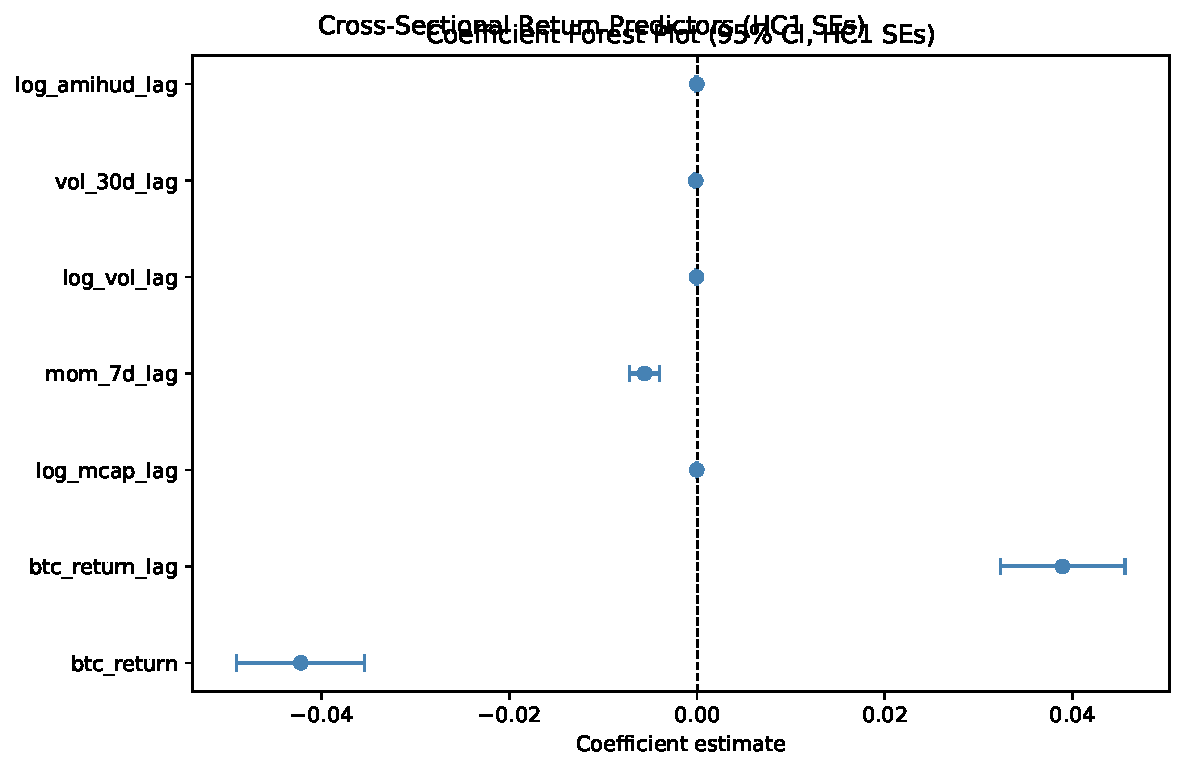
\includegraphics[width=0.75\textwidth]{../figures/cross_section_coef.pdf}
\caption{Coefficient Estimates for Cross-Sectional Model (HC1)}
\label{fig:cross_coef}
\end{figure}

\subsection{Robustness of Standard Errors}

Columns (3)--(5) of Table~\ref{tab:cross_section} show the same specification
with three different covariance estimators: HC1 (White), HC3 (bias-corrected),
and HAC (Newey-West with 5 lags). The qualitative conclusions are unchanged,
though HAC standard errors are generally larger, reflecting the time-series
dependence in the pooled panel.

\section{Fama-MacBeth Regressions}

We run monthly cross-sectional regressions of next-month returns on lagged
characteristics. The Fama-MacBeth $t$-statistic accounts for time-series
variation in coefficient estimates.

\begin{table}[H]
\centering
\caption{Fama-MacBeth Cross-Sectional Regressions}
\label{tab:fm}
\begin{threeparttable}
\begin{tabular}{l cccc}
\toprule
Variable & $\bar{\gamma}$ & FM $t$ & $p$-value & Months \\
\midrule
Monthly Return & -0.03401 & -2.51 & 0.013 & 135 \\
Avg Mcap & -0.00241 & -0.83 & 0.409 & 135 \\
Avg Volume & -0.00034 & -0.14 & 0.889 & 135 \\
Avg Vol & -0.00795 & -2.25 & 0.026 & 135 \\
\bottomrule
\end{tabular}
\begin{tablenotes}
\footnotesize
\item $\bar{\gamma}$ is the time-series average of monthly cross-sectional
      slope coefficients. The FM $t$-statistic uses the standard error
      $\text{sd}(\hat{\gamma}_t) / \sqrt{T}$.
\end{tablenotes}
\end{threeparttable}
\end{table}

\begin{figure}[H]
\centering
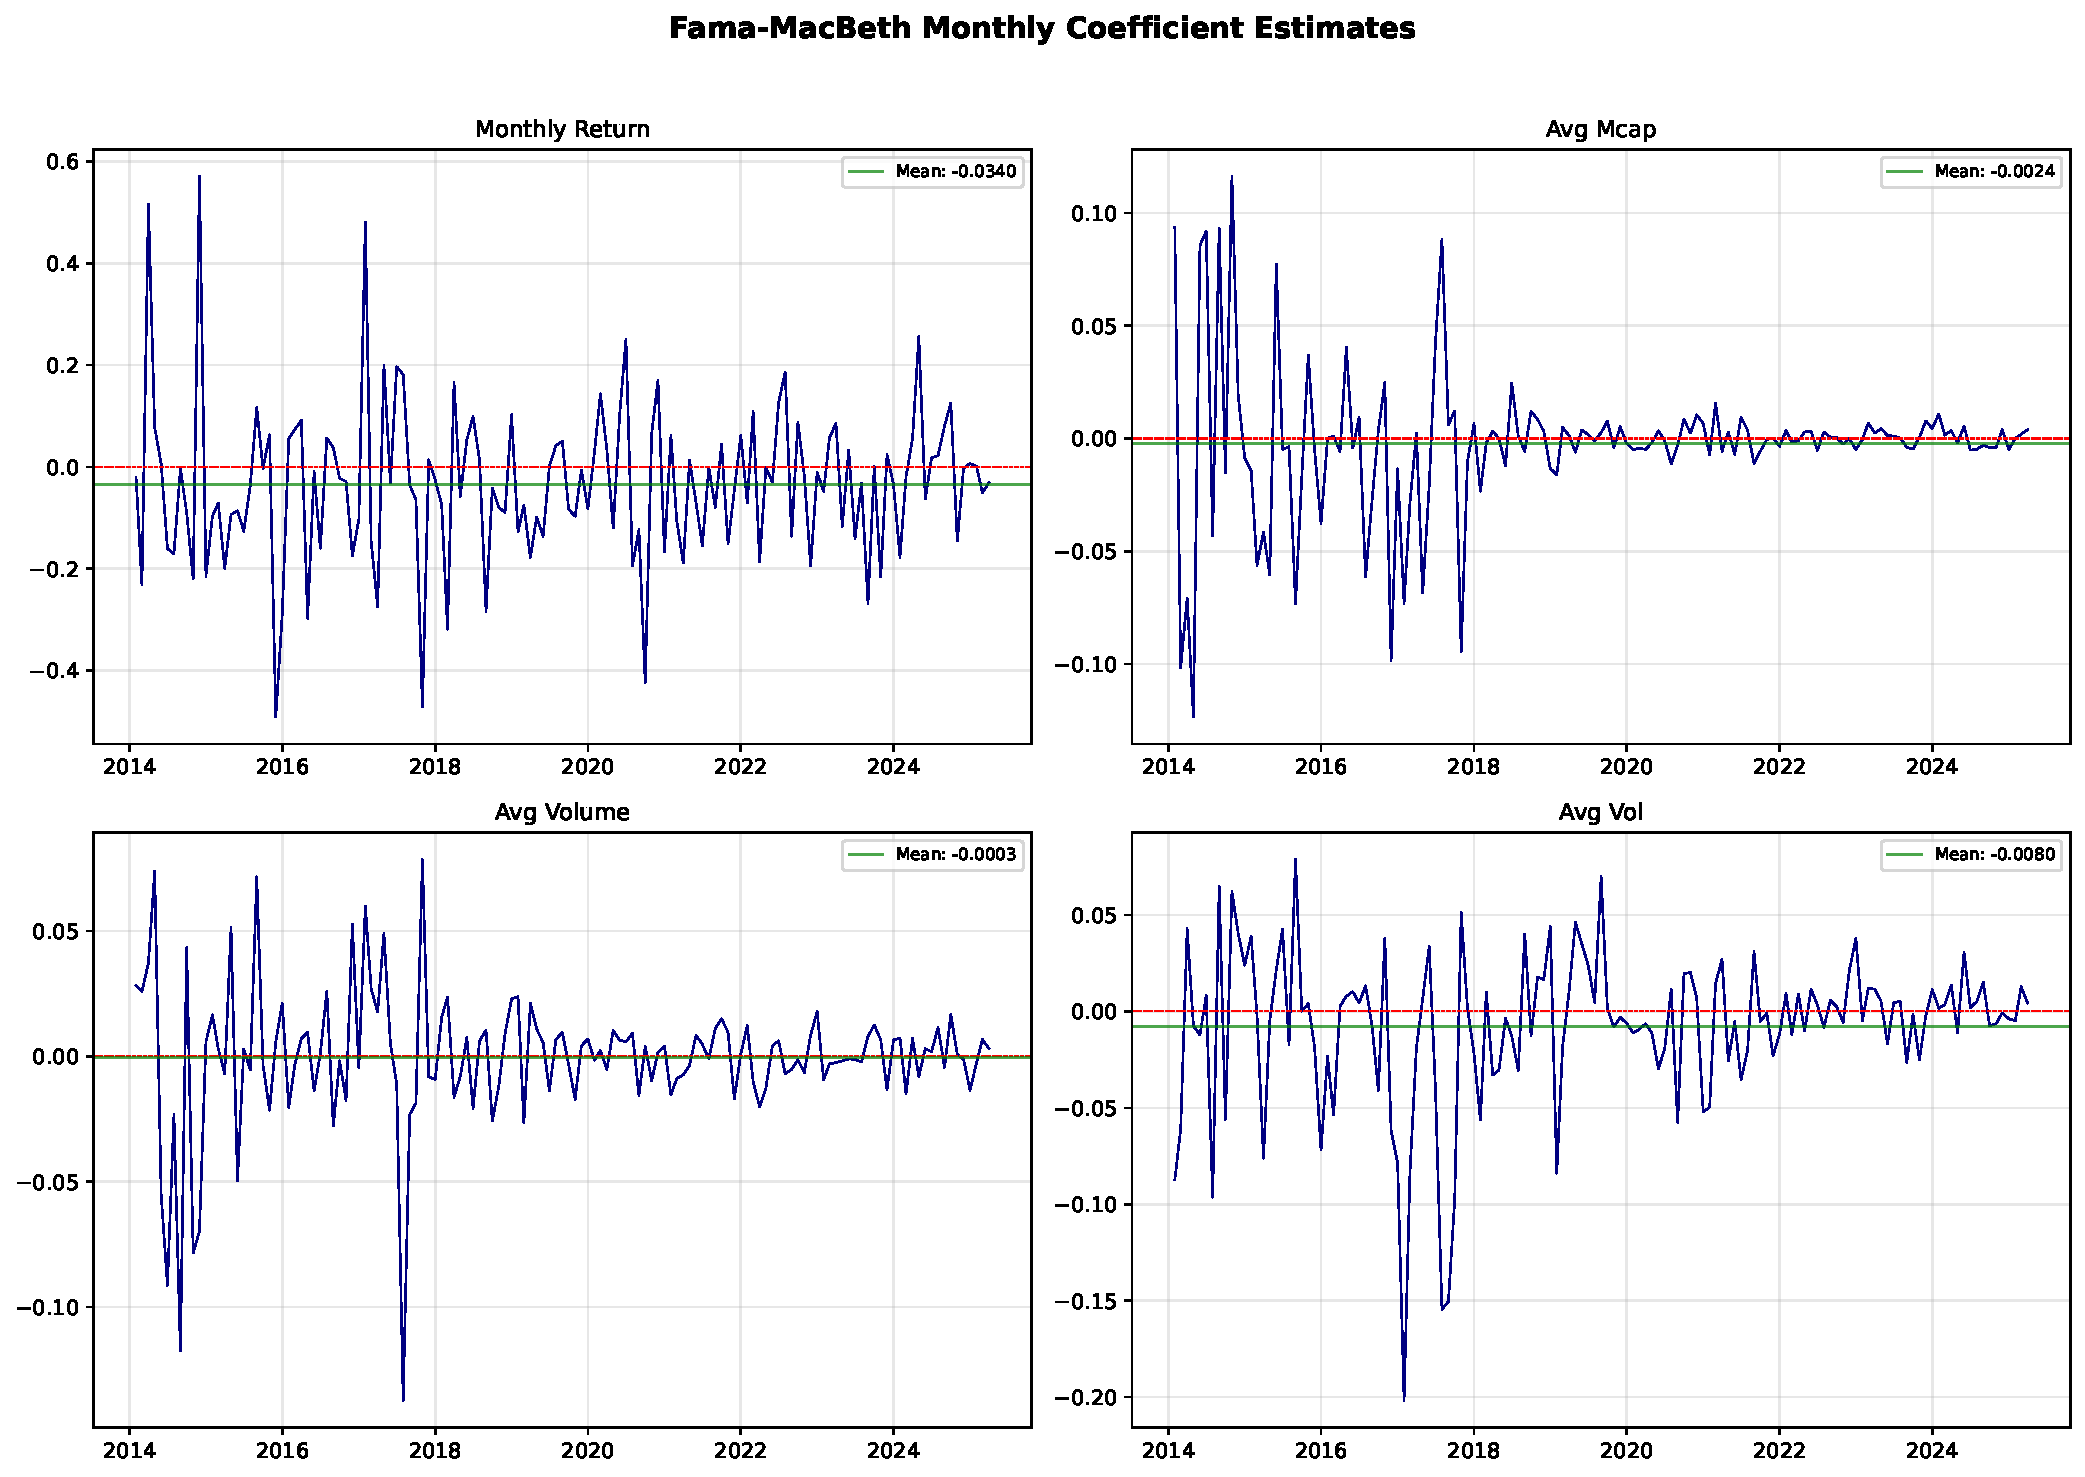
\includegraphics[width=\textwidth]{../figures/fama_macbeth_coefs.pdf}
\caption{Time-Varying Fama-MacBeth Coefficient Estimates}
\label{fig:fm_coefs}
\end{figure}

\begin{figure}[H]
\centering
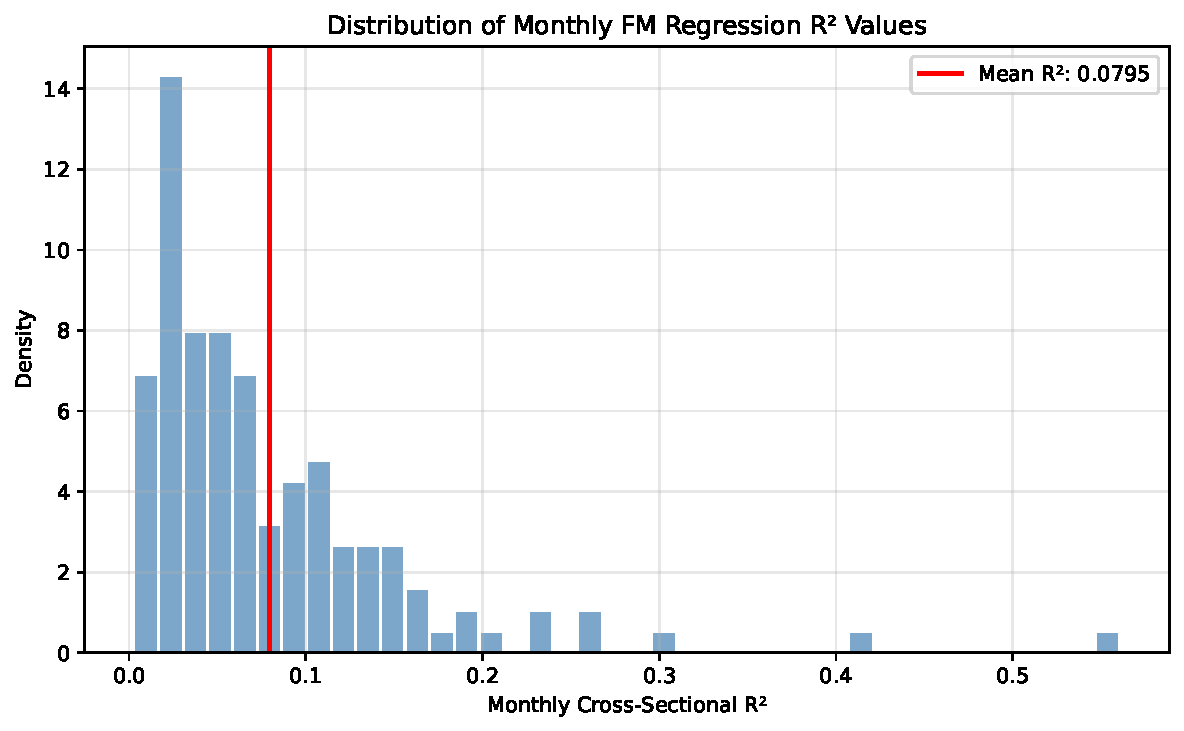
\includegraphics[width=0.7\textwidth]{../figures/fm_r_squared_dist.pdf}
\caption{Distribution of Monthly Cross-Sectional $R^2$}
\label{fig:fm_r2}
\end{figure}

\section{Volatility Spillovers}

We test for BTC-to-altcoin volatility transmission using squared returns
as a proxy for conditional variance. The spillover coefficient captures
the extent to which BTC volatility shocks propagate to altcoin markets.

The contemporaneous BTC squared return is highly significant in explaining
altcoin squared returns, confirming strong volatility spillover effects.
Lagged BTC volatility also contributes, suggesting persistent transmission.

\section{Residual Diagnostics}

\begin{figure}[H]
\centering
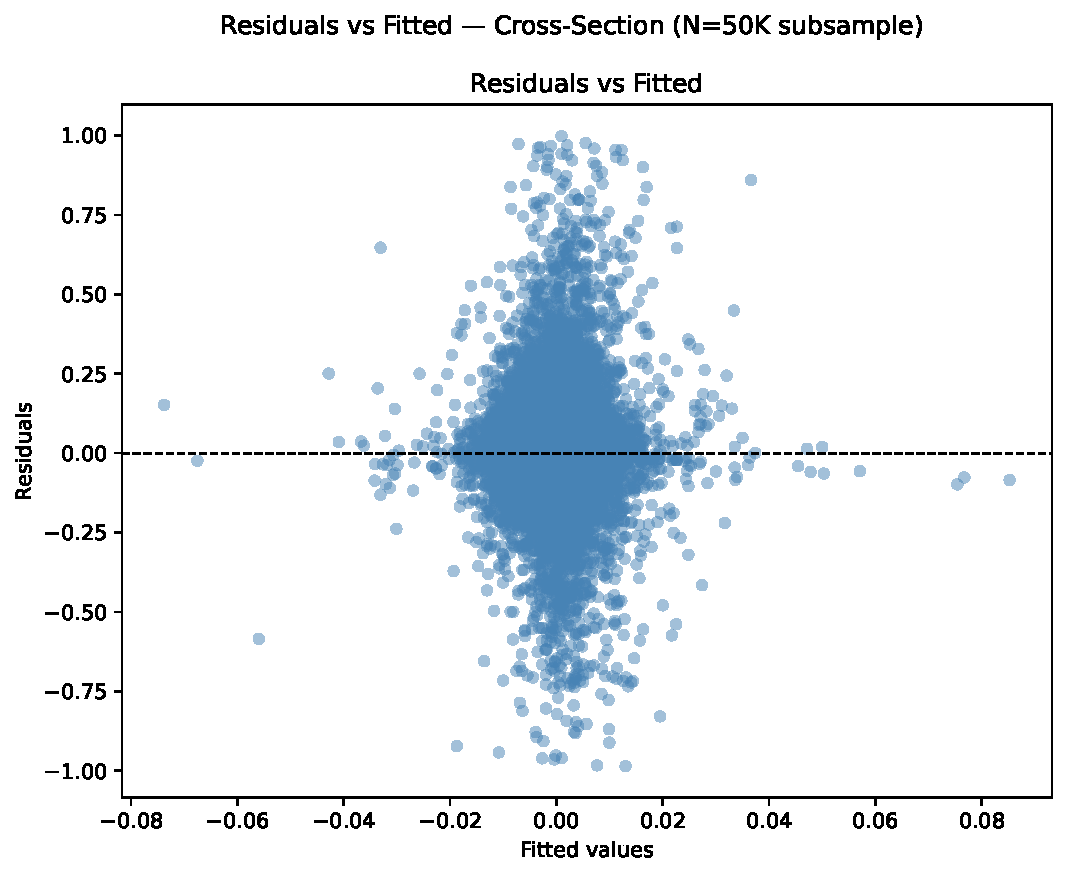
\includegraphics[width=0.85\textwidth]{../figures/cross_section_resid.pdf}
\caption{Residuals vs Fitted --- Cross-Section Full Model}
\label{fig:cross_resid}
\end{figure}

The residual plots confirm massive heteroskedasticity (as expected with
financial returns data) and heavy tails, validating our use of
heteroskedasticity-robust standard errors throughout.

\section{Conclusion}

The cross-section of cryptocurrency returns is dominated by market-wide
co-movement with Bitcoin. Individual coin characteristics (size, momentum,
volume, illiquidity) have limited incremental predictive power for
next-period returns, consistent with a relatively efficient market.
However, the strong volatility spillover from BTC to altcoins has
important implications for risk management and portfolio construction.

\end{document}
